\documentclass[main.tex]{subfiles} % Subfile-Class


% ============================================================================== %
%                            Subfile document                                    %
% ============================================================================== %

\begin{document}

\subsection{Risikomanagement}

Das Risikomanagement wird nach der ALARP-Methode (\textit{engl. as low as
    reasonable possible}) durchgeführt. Dafür werden Risiken im ersten Schritt
detektiert und in einem nächsten Schritt durch Risikovermindernde Massnahmen
auf ein Mass reduziert, welche ein vernünftiges Mass für Sicherheit bietet. Die
Bewertung wird mit dem gesamten Team auf der subjektiven Einschätzung auf die
Erfüllung der Aufgabe gestützt. Ziel ist es, zu einem möglichst frühen
Zeitpunkt des Projektes kritisches Punkte des Projektes zu identifizieren und
den Fokus auf entsprechende Punkte zu legen. \\

% -------------------------------------- Erläuterung Bewertung

\subsubsection*{Eintrittswahrscheinlichkeit (EW)}

Die Eintrittswahrscheinlichkeit ist ein Mass für die wahscheinlichkeit, mit
welcher ein Ereignis eintreten könnte.

\begin{table}[H]
    \begin{tabularx}{\textwidth}{|>{\centering\arraybackslash}p{1cm}|>{\raggedright\arraybackslash}X|>{\centering\arraybackslash}p{2cm}|}
        \hline
        \textbf{EW} & \textbf{Bezeichnung} & \textbf{\%} \\
        \hline
        6           & häufig               & $>90\%$     \\
        \hline
        5           & wahscheinlich        & $>70\%$     \\
        \hline
        4           & gelegentlich         & $>50\%$     \\
        \hline
        3           & entfernt vorstellbar & $>30\%$     \\
        \hline
        2           & unwahrscheinlich     & $>15\%$     \\
        \hline
        1           & unvorstellbar        & $>5\%$      \\
        \hline
        %  >> neue Zeilen <<
        %    &  &  \\
        %    \hline

    \end{tabularx}
    \caption{Legende Eintrittswahrscheinlichkeit}~\label{tab:Legende_Eintrittswahrscheinlichkeit}
\end{table}

\subsubsection*{Schadensausmass (SA)}

Das Schadensausmass ist ein Mass dafür, wie fatal ein eintretends Ereignis für
den Projekterfolg ist.

\begin{table}[H]
    \begin{tabularx}{\textwidth}{|>{\centering\arraybackslash}p{1cm}|>{\raggedright\arraybackslash}X|>{\raggedright\arraybackslash}X|}
        \hline
        \textbf{SA} & \textbf{Bezeichnung} & \textbf{Auswirkung}          \\
        \hline
        4           & katastrophal         & Wettbewerb abgebrochen       \\
        \hline
        3           & kritisch             & Gefährdung für Projekterfolg \\
        \hline
        2           & geringfügig          & Minderung des Projekterfolgs \\
        \hline
        1           & unwesentlich         & Störung des Projekterfolgs   \\
        \hline
        %  >> neue Zeilen <<
        %    &  &  \\
        %    \hline
    \end{tabularx}
    \caption{Legende Schadensausmass}~\label{tab:Legende_Schadensausmass}
\end{table}

\subsubsection*{Bereichsdefinition}

Die entsprechenden Risiken sind mit der folgenden Colorierung farbig Codiert,
um die Notwendigkeit von Massnahmen zu kennzeichnen.

\begin{table}[H]
    \centering
    \begin{tabular}{|c|c|}
        \hline
        Farbcodierung         & Bedeutung             \\
        \hline
        \cellcolor{green!30}  & Akzeptabler Bereich   \\
        \hline
        \cellcolor{yellow!30} & ALARP-Bereich         \\
        \hline
        \cellcolor{red!30}    & Inakzeptabler Bereich \\
        \hline
    \end{tabular}
    \caption{Legende Bereichsdefinition}~\label{tab:Legende_Bereichsdefinition}
\end{table}

% -------------------------------------- Tabelle Massnahmen

\subsection{Erfasste Risiken}

Die nachfolgenden Tabellen zeigen die identifizierten Risiken bis zum aktuellen
Zeitpunkt. \\

% ========= ALLGEMEIN

\subsubsection*{Allgemeines}

\newcounter{Erfasste_Risiken_counter_allg} % define Rowcounter
\setcounter{Erfasste_Risiken_counter_allg}{0}

\begin{table}[H]
    \begin{tabularx}{\textwidth}{|>{\centering\arraybackslash}p{0.5cm}|>{\raggedright\arraybackslash}X|>{\centering\arraybackslash}p{0.75cm}|>{\centering\arraybackslash}p{0.75cm}|>{\raggedright\arraybackslash}X|}
        \hline
        \textbf{\#} & \textbf{Risiko} & \textbf{SA} & \textbf{EW} & \textbf{Auswirkungen} \\

        \hline
        \rowcolor{yellow!30}
        \refstepcounter{Erfasste_Risiken_counter_allg}~\label{tabrow:risks_1_1}1.\arabic{Erfasste_Risiken_counter_allg}
                    &                 &             &             &                       \\

        \hline
    \end{tabularx}
    \caption{Erfasste Risiken mit Bewertung}~\label{tab:Erfasste_Risiken_allg}
\end{table}

% ========= MECHANIK
\subsubsection*{Mechanik}

\newcounter{Erfasste_Risiken_counter_mech} % define Rowcounter
\setcounter{Erfasste_Risiken_counter_mech}{0}

\begin{table}[H]
    \begin{tabularx}{\textwidth}{|>{\centering\arraybackslash}p{0.5cm}|>{\raggedright\arraybackslash}X|>{\centering\arraybackslash}p{0.75cm}|>{\centering\arraybackslash}p{0.75cm}|>{\raggedright\arraybackslash}X|}
        \hline
        \textbf{\#} & \textbf{Risiko}                                                                       & \textbf{SA} & \textbf{EW} & \textbf{Auswirkungen}    \\

        \hline
        \rowcolor{yellow!30}
        \refstepcounter{Erfasste_Risiken_counter_mech}~\label{tabrow:risks_2_1}2.\arabic{Erfasste_Risiken_counter_mech}
                    & Fahrzeug kann Hindernis erfassen und aufnehmen, aber nicht genau genug positionieren. & 3           & 4           & Punktabzug bei Bewertung \\

        \hline
        \rowcolor{red!30}
        \refstepcounter{Erfasste_Risiken_counter_mech}~\label{tabrow:risks_2_2}2.\arabic{Erfasste_Risiken_counter_mech}
                    & Fahrzeug überschreitet zugelassenes Gesamtgewicht, 2kg ist ein enger Rahmen.          & 4           & 3           & Disqualifizierung        \\

    \end{tabularx}
    \caption{Erfasste Risiken aus dem Maschinenbau-Bereich}~\label{tab:Erfasste_Risiken_mech}

\end{table}

% ========= ELEKTRO
\subsubsection*{Elektrotechnik}

\newcounter{Erfasste_Risiken_counter_elektro} % define Rowcounter
\setcounter{Erfasste_Risiken_counter_elektro}{0}

\begin{table}[H]
    \begin{tabularx}{\textwidth}{|>{\centering\arraybackslash}p{0.5cm}|>{\raggedright\arraybackslash}X|>{\centering\arraybackslash}p{0.75cm}|>{\centering\arraybackslash}p{0.75cm}|>{\raggedright\arraybackslash}X|}
        \hline
        \textbf{\#} & \textbf{Risiko}                                                                                & \textbf{SA} & \textbf{EW} & \textbf{Auswirkungen}                                                     \\

        \hline
        \rowcolor{red!30}
        \refstepcounter{Erfasste_Risiken_counter_elektro}~\label{tabrow:risks_3_1}3.\arabic{Erfasste_Risiken_counter_elektro}
                    & Fahrzeug kann Linie nicht erkennen und kommt deshalb von Linie ab                              & 4           & 5           & Disqualifizierung                                                         \\

        \hline
        \rowcolor{red!30}
        \refstepcounter{Erfasste_Risiken_counter_elektro}~\label{tabrow:risks_3_2}3.\arabic{Erfasste_Risiken_counter_elektro}
                    & Fahrzeug wird durch Lichtverhältnisse durch Umwelteinflüsse gestört.                           & 3           & 6           & Punktabzug durch abkommen von der Linie oder Kollisionen mit Hindernissen \\

        \hline
        \rowcolor{yellow!30}
        \refstepcounter{Erfasste_Risiken_counter_elektro}~\label{tabrow:risks_3_3}3.\arabic{Erfasste_Risiken_counter_elektro}
                    & Akku reicht nicht aus für beide Läufe mit Tests, da aufgrund von Gewicht zu eng dimensioniert. & 4           & 2           & Fahrzeug kann nicht in Ziel ankommen.                                     \\

        \hline
        \rowcolor{yellow!30}
        \refstepcounter{Erfasste_Risiken_counter_elektro}~\label{tabrow:risks_3_4}3.\arabic{Erfasste_Risiken_counter_elektro}
                    & Kommunikation verschiedener Microcontroller mit Hauptrechner gestört durch Umwelteinflüsse.    & 3           & 2           & Unter umständen falsche/keine Steuersignale                               \\
        \hline

    \end{tabularx}
    \caption{Erfasste Risiken aus dem Elektrotechnik-Bereich}~\label{tab:Erfasste_Risiken_elektro}

\end{table}

% ========= INFORMATIK
\subsubsection*{Informatik}

\newcounter{Erfasste_Risiken_counter_info} % define Rowcounter
\setcounter{Erfasste_Risiken_counter_info}{0}

\begin{table}[H]
    \begin{tabularx}{\textwidth}{|>{\centering\arraybackslash}p{0.5cm}|>{\raggedright\arraybackslash}X|>{\centering\arraybackslash}p{0.75cm}|>{\centering\arraybackslash}p{0.75cm}|>{\raggedright\arraybackslash}X|}
        \hline
        \textbf{\#} & \textbf{Risiko}                                                                   & \textbf{SA} & \textbf{EW} & \textbf{Auswirkungen}                                  \\

        \hline
        \rowcolor{red!30}
        \refstepcounter{Erfasste_Risiken_counter_info}~\label{tabrow:risks_4_1}4.\arabic{Erfasste_Risiken_counter_info}
                    & Fahrzeug verliert Orientierung im Parcours und kann deshalb Ziel nicht erreichen. & 3           & 5           & Fahrzeug braucht lange, bis es Ziel zufällig erreicht. \\

    \end{tabularx}
    \caption{Erfasste Risiken aus dem Informatik-Bereich}~\label{tab:Erfasste_Risiken_info}
\end{table}

% ============================================ Massnahmen ======================================================

\subsubsection{Erfasste Massnahmen}

% ========= ALLGEMEIN

\subsubsection*{Allgemein}

\begin{table}[H]
    \begin{tabularx}{\textwidth}{|>{\centering\arraybackslash}p{2cm}|>{\raggedright\arraybackslash}X|>{\centering\arraybackslash}p{0.75cm}|}
        \hline
        \textbf{Risiko \#} & \textbf{Massnahme}
                           & \textbf{Neu EW}    \\

        \hline
        \rowcolor{yellow!30}
        1.~\ref{}          &
                           &                    \\
        \\
        \hline

    \end{tabularx}
    \caption{Erfasste Massnahmen Allgemein betreffende Risiken}~\label{tab:Erfasste_Massnahmen_allg}
\end{table}

Abbildung~\ref{fig:Diagramm_Risiko_allg} zeigt schematisch auf, wie die
getroffenen Massnahmen entsprechende Risiken auf den Projekterfolg reduzieren.

\begin{figure}[h]
    \centering
    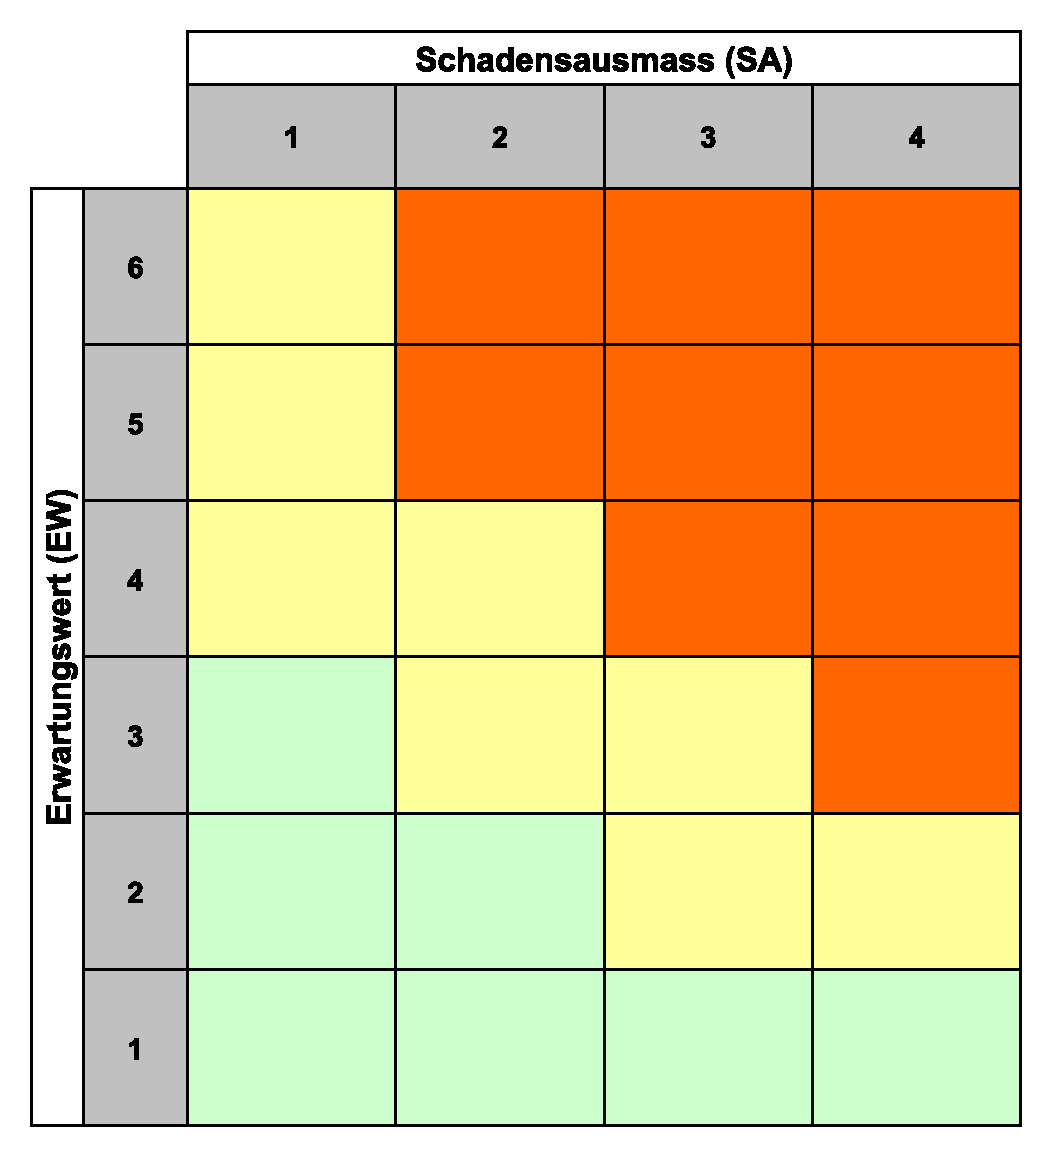
\includegraphics[width=0.5\textwidth]{./Risks_Diagramm/Diagramm_Risiko_allg.pdf}
    \caption{Grafische Darstellung Risikoanalyse Allgemein}
    \label{fig:Diagramm_Risiko_allg}
\end{figure}

% ========= MECHANIK

\subsubsection*{Mechanik}

\begin{table}[H]
    \begin{tabularx}{\textwidth}{|>{\centering\arraybackslash}p{2cm}|>{\raggedright\arraybackslash}X|>{\centering\arraybackslash}p{0.75cm}|}
        \hline
        \textbf{Risiko \#}        & \textbf{Massnahme}
                                  & \textbf{Neu EW}                                                                                                                                                               \\                                                                                                                                                                                                 \\

        \hline
        \rowcolor{yellow!30}
        2.~\ref{tabrow:risks_2_1} & Höhere Gewichtung auf dieses Detail in der Konzeptbewertung.
                                  & 3                                                                                                                                                                             \\

        \hline
        \rowcolor{green!30}
        2.~\ref{tabrow:risks_2_2} & Gewicht der Bauteile frühzeitig überschlagen und bei jedem Entwicklungsschritt berücksichtigen. Liste führen für schon bekannte Gewichte und Budget für Baugruppen festlegen.
                                  & 1                                                                                                                                                                             \\

        \hline

    \end{tabularx}
    \caption{Erfasste Massnahmen Maschinenbau betreffende Risiken}~\label{tab:Erfasste_Massnahmen_mech}
\end{table}

Abbildung~\ref{fig:Diagramm_Risiko_mechanik} zeigt schematisch auf, wie die
getroffenen Massnahmen entsprechende Risiken auf den Projekterfolg reduzieren.

\begin{figure}[h]
    \centering
    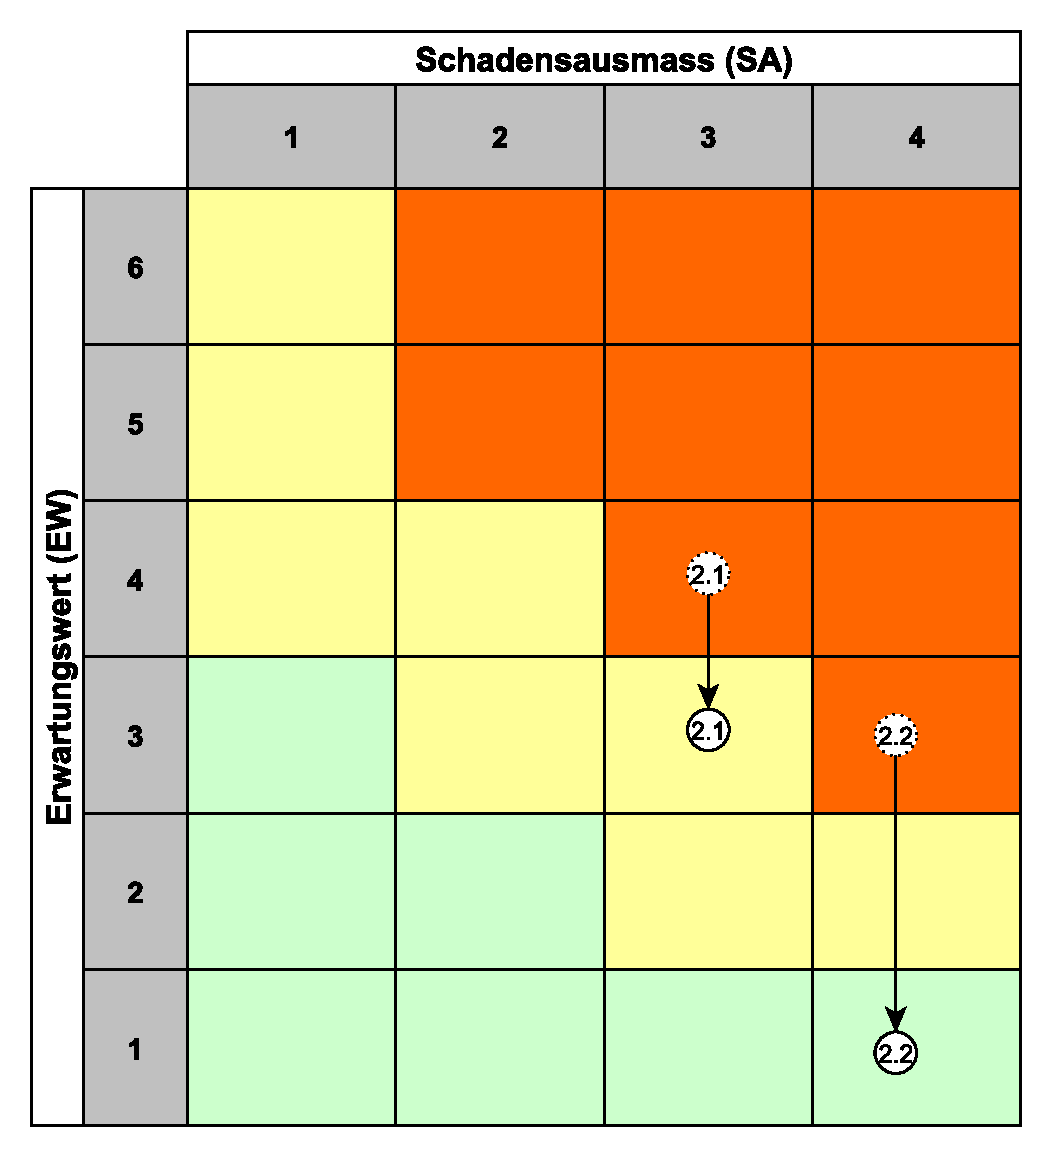
\includegraphics[width=0.5\textwidth]{./Risks_Diagramm/Diagramm_Risiko_mechanik.pdf}
    \caption{Grafische Darstellung Risikoanalyse Maschinenbau}
    \label{fig:Diagramm_Risiko_mechanik}
\end{figure}

% ========= ELEKTRONIK

\subsubsection*{Elektrotechnik}

\begin{table}[H]
    \begin{tabularx}{\textwidth}{|>{\centering\arraybackslash}p{2cm}|>{\raggedright\arraybackslash}X|>{\centering\arraybackslash}p{0.75cm}|}
        \hline
        \textbf{Risiko \#}        & \textbf{Massnahme}
                                  & \textbf{Neu EW}                                                                                                                                                                                        \\

        \hline
        \rowcolor{yellow!30}
        3.~\ref{tabrow:risks_3_1} & Frühzeitiges Testen und optimieren der Genauigkeit der Sensorik. Möglichkeit bieten, nach Fahrzeugwinkel und gefahrener Strecke Fahrzeug zu Regeln. Technologieentscheid erst nach ausgiebigem Testen.
                                  & 2                                                                                                                                                                                                      \\

        \hline
        \rowcolor{yellow!30}
        3.~\ref{tabrow:risks_3_2} & Sensorik, welche optisch arbeitet, möglichst abgekapselt von Umwelt betreiben. Alternativ Wellenlängen, die das sichtbare Licht beinhalten, vermeiden.
                                  & 3                                                                                                                                                                                                      \\

        \hline
        \rowcolor{green!30}
        3.~\ref{tabrow:risks_3_3} & Akku doppelt herstellen/einkaufen, Ladestation extern ausführen um immer einen voll geladenen Akku bereit zu haben.
                                  & 1                                                                                                                                                                                                      \\

        \hline
        \rowcolor{green!30}
        3.~\ref{tabrow:risks_3_4} & Kommunikationsleitungen mindestens als twisted-Pairs mit GND - besser aber geschirmt ausführen.
                                  & 1                                                                                                                                                                                                      \\

        \hline

    \end{tabularx}
    \caption{Erfasste Massnahmen für Risikoanalyse}~\label{tab:Erfasste_Massnahmen}
\end{table}

Abbildung~\ref{fig:Diagramm_Risiko_elektro} zeigt schematisch auf, wie die
getroffenen Massnahmen entsprechende Risiken auf den Projekterfolg reduzieren.

\begin{figure}[h]
    \centering
    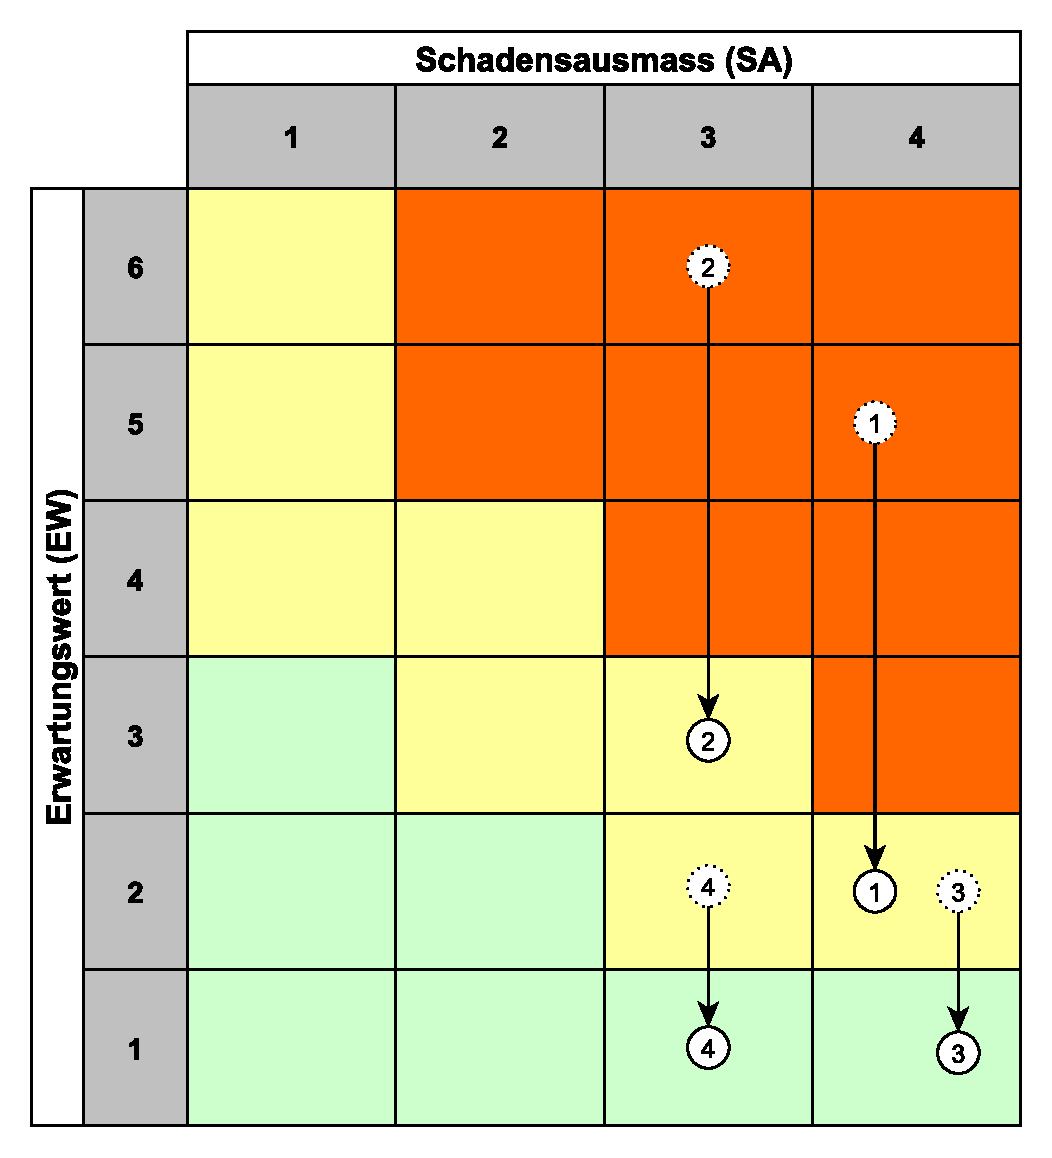
\includegraphics[width=0.5\textwidth]{./Risks_Diagramm/Diagramm_Risiko_elektro.pdf}
    \caption{Grafische Darstellung Risikoanalyse Elektrotechnik}
    \label{fig:Diagramm_Risiko_elektro}
\end{figure}

% ========= INFORMATIK

\subsubsection*{Informatik}

\begin{table}[H]
    \begin{tabularx}{\textwidth}{|>{\centering\arraybackslash}p{2cm}|>{\raggedright\arraybackslash}X|>{\centering\arraybackslash}p{0.75cm}|}
        \hline
        \textbf{Risiko \#}        & \textbf{Massnahme}
                                  & \textbf{Neu EW}                             \\

        \hline
        \rowcolor{yellow!30}
        4.~\ref{tabrow:risks_4_1} & Fallbacklösung, Fahrzeug fährt immer links.
                                  & 3                                           \\

        \hline

    \end{tabularx}
    \caption{Erfasste Massnahmen für Risikoanalyse}~\label{tab:Erfasste_Massnahmen}
\end{table}

Abbildung~\ref{fig:Diagramm_Risiko_info} zeigt schematisch auf, wie die
getroffenen Massnahmen entsprechende Risiken auf den Projekterfolg reduzieren.

\begin{figure}[h]
    \centering
    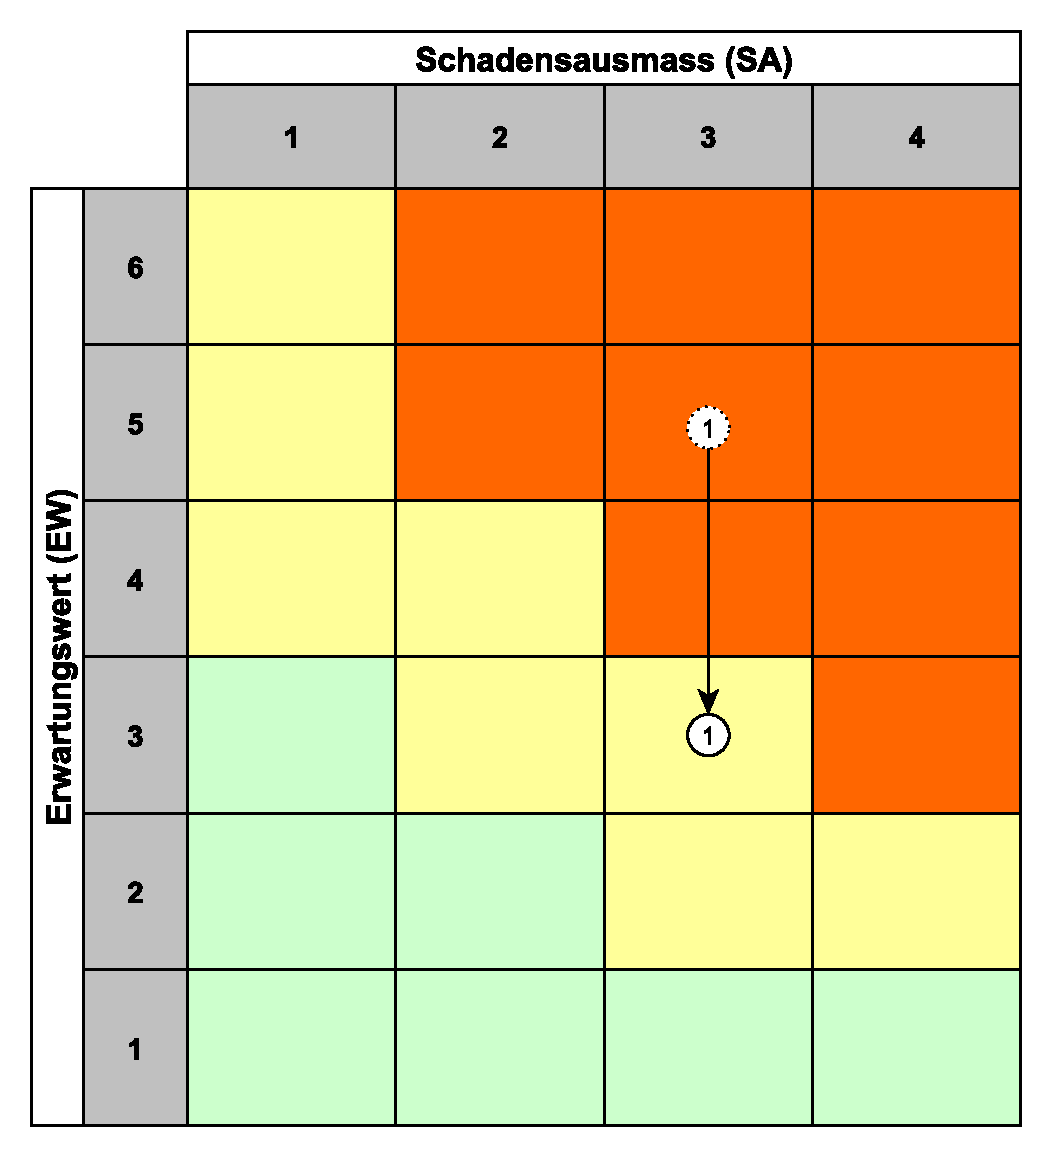
\includegraphics[width=0.5\textwidth]{./Risks_Diagramm/Diagramm_Risiko_info.pdf}
    \caption{Grafische Darstellung Risikoanalyse Informatik}
    \label{fig:Diagramm_Risiko_info}
\end{figure}

\end{document}
